\documentclass[11pt,oneside]{article}
\usepackage[T1]{fontenc}
\usepackage[utf8]{inputenc}
% \usepackage{lmodern}
%\usepackage[adobe-utopia,uppercase=upright,greeklowercase=upright]{mathdesign}
\usepackage[adobe-utopia]{mathdesign}
%\usepackage{minionpro}
% \usepackage{pifont}
% \usepackage{amssymb}
\usepackage{amsmath}
\usepackage[francais]{babel}
% \usepackage[francais]{varioref}
\usepackage[dvips]{graphicx}

\usepackage{framed}
\usepackage[normalem]{ulem}
\usepackage{fancyhdr}
\usepackage{titlesec}
\usepackage{vmargin}
\usepackage{longtable}

\usepackage{ifthen}


%\usepackage{epsfig}
\usepackage{subfig}

\usepackage{multirow}
\usepackage{multicol} % Portions de texte en colonnes
\usepackage{flafter}%floatants après la référence



\usepackage{color}
\usepackage{colortbl}


\definecolor{gris25}{gray}{0.75}
\definecolor{bleu}{RGB}{18,33,98}
\definecolor{bleuf}{RGB}{42,94,171}
\definecolor{bleuc}{RGB}{231,239,247}
\definecolor{rougef}{RGB}{185,18,27}
\definecolor{rougec}{RGB}{255,230,231}
\definecolor{vertf}{RGB}{103,126,82}
\definecolor{vertc}{RGB}{220,255,191}
\definecolor{violetf}{RGB}{112,48,160}
\definecolor{violetc}{RGB}{230,224,236}

\newenvironment{sci}[1][\hsize]%
{%
    \def\FrameCommand%
    {%
%\rotatebox{90}{\textit{\textsf{Scilab}}\includegraphics[height=.8cm]{png/logo_scilab}} 
\rotatebox{90}{\includegraphics[height=.6cm]{png/logo_scilab}} 
        {\color{violetf}\vrule width 3pt}%
        \hspace{0pt}%must no space.
        \fboxsep=\FrameSep\colorbox{violetc}%
    }%
    \MakeFramed{\hsize #1 \advance\hsize-\width\FrameRestore}%
}%
{\endMakeFramed}%

\newenvironment{pseudo}[1][\hsize]%
{%
    \def\FrameCommand%
    {%
\rotatebox{90}{\textit{\textsf{Pseudo Code}}} 
        {\color{violetf}\vrule width 3pt}%
        \hspace{0pt}%must no space.
        \fboxsep=\FrameSep\colorbox{violetc}%
    }%
    \MakeFramed{\hsize #1 \advance\hsize-\width\FrameRestore}%
}%
{\endMakeFramed}%

\newenvironment{py}[1][\hsize]%
{%
    \def\FrameCommand%
    {%
%\rotatebox{90}{\textit{\textsf{Python}}} 
\rotatebox{90}{\includegraphics[height=.6cm]{png/logo_python}} 
        {\color{violetf}\vrule width 3pt}%
        \hspace{0pt}%must no space.
        \fboxsep=\FrameSep\colorbox{violetc}%
    }%
    \MakeFramed{\hsize #1 \advance\hsize-\width\FrameRestore}%
}%
{\endMakeFramed}%


\newenvironment{corrige}[1][\hsize]%
{%
    \def\FrameCommand
    {%
\rotatebox{90}{\textit{\textsf{Correction}}} 
        {\color{violetf}\vrule width 3pt}%
        \hspace{0pt}%must no space.
        \fboxsep=\FrameSep\colorbox{violetc}%
    }%
    \MakeFramed{\hsize#1\advance\hsize-\width\FrameRestore}%
}%
{\endMakeFramed}%



\newenvironment{rem}[1][\hsize]%
{%
    \def\FrameCommand
    {%
\rotatebox{90}{\textit{\textsf{Remarque}}} 
        {\color{bleuf}\vrule width 3pt}%
        \hspace{0pt}%must no space.
        \fboxsep=\FrameSep\colorbox{bleuc}%
    }%
    \MakeFramed{\hsize#1\advance\hsize-\width\FrameRestore}%
}%
{\endMakeFramed}%


\newenvironment{savoir}[1][\hsize]%
{%
    \def\FrameCommand
    {%
\rotatebox{90}{\textit{\textsf{Savoir}}} 
        {\color{bleuf}\vrule width 3pt}%
        \hspace{0pt}%must no space.
        \fboxsep=\FrameSep\colorbox{bleuc}%
    }%
    \MakeFramed{\hsize#1\advance\hsize-\width\FrameRestore}%
}%
{\endMakeFramed}%

\newenvironment{prob}[1][\hsize]%
{%
    \def\FrameCommand%
    {%
\rotatebox{90}{\textit{\textsf{ Problématique}}} 
        {\color{rougef}\vrule width 3pt}%
        \hspace{0pt}%must no space.
        \fboxsep=\FrameSep\colorbox{rougec}%
    }%
    \MakeFramed{\hsize#1\advance\hsize-\width\FrameRestore}%
}%
{\endMakeFramed}%

\newenvironment{obj}[1][\hsize]%
{%
    \def\FrameCommand%
    {%
\rotatebox{90}{\textit{\textsf{ $\;$}}} 
        {\color{rougef}\vrule width 3pt}%
        \hspace{0pt}%must no space.
        \fboxsep=\FrameSep\colorbox{rougec}%
    }%
    \MakeFramed{\hsize#1\advance\hsize-\width\FrameRestore}%
}%
{\endMakeFramed}%

\newenvironment{defi}[1][\hsize]%
{%
    \def\FrameCommand%
    {%
\rotatebox{90}{\textit{\textsf{Définition\\}}} 
        {\color{bleuf}\vrule width 3pt}%
        \hspace{0pt}%must no space.
        \fboxsep=\FrameSep\colorbox{bleuc}%
    }%
    \MakeFramed{\hsize#1\advance\hsize-\width\FrameRestore}%
}%
{\endMakeFramed}%


\newenvironment{demo}[1][\hsize]%
{%
    \def\FrameCommand%
    {%
\rotatebox{90}{\textit{\textsf{Démonstration\\}}} 
        {\color{bleuf}\vrule width 3pt}%
        \hspace{0pt}%must no space.
        \fboxsep=\FrameSep\colorbox{bleuc}%
    }%
    \MakeFramed{\hsize#1\advance\hsize-\width\FrameRestore}%
}%
{\endMakeFramed}%


\newenvironment{hypo}[1][\hsize]%
{%
    \def\FrameCommand%
    {%
\rotatebox{90}{\textit{\textsf{Hypothèse\\}}} 
        {\color{bleuf}\vrule width 3pt}%
        \hspace{0pt}%must no space.
        \fboxsep=\FrameSep\colorbox{bleuc}%
    }%
    \MakeFramed{\hsize#1\advance\hsize-\width\FrameRestore}%
}%
{\endMakeFramed}%


\newenvironment{prop}[1][\hsize]%
{%
    \def\FrameCommand%
    {%
\rotatebox{90}{\textit{\textsf{Propriété\\}}} 
        {\color{bleuf}\vrule width 3pt}%
        \hspace{0pt}%must no space.
        \fboxsep=\FrameSep\colorbox{bleuc}%
    }%
    \MakeFramed{\hsize#1\advance\hsize-\width\FrameRestore}%
}%
{\endMakeFramed}%

\newenvironment{props}[1][\hsize]%
{%
    \def\FrameCommand%
    {%
\rotatebox{90}{\textit{\textsf{Propriétés\\}}} 
        {\color{bleuf}\vrule width 3pt}%
        \hspace{0pt}%must no space.
        \fboxsep=\FrameSep\colorbox{bleuc}%
    }%
    \MakeFramed{\hsize#1\advance\hsize-\width\FrameRestore}%
}%
{\endMakeFramed}%

\newenvironment{exemple}[1][\hsize]%
{%
    \def\FrameCommand%
    {%
\rotatebox{90}{\textit{\textsf{Exemple\\}}} 
        {\color{vertf}\vrule width 3pt}%
        \hspace{0pt}%must no space.
        \fboxsep=\FrameSep\colorbox{vertc}%
    }%
    \MakeFramed{\hsize#1\advance\hsize-\width\FrameRestore}%
}%
{\endMakeFramed}%

\newenvironment{resultat}[1][\hsize]%
{%
    \def\FrameCommand%
    {%
\rotatebox{90}{\textit{\textsf{Résultat\\}}} 
        {\color{rougef}\vrule width 3pt}%
        \hspace{0pt}%must no space.
        \fboxsep=\FrameSep\colorbox{rougec}%
    }%
    \MakeFramed{\hsize#1\advance\hsize-\width\FrameRestore}%
}%
{\endMakeFramed}%

\newenvironment{methode}[1][\hsize]%
{%
    \def\FrameCommand%
    {%
\rotatebox{90}{\textit{\textsf{Méthode\\}}} 
        {\color{rougef}\vrule width 3pt}%
        \hspace{0pt}%must no space.
        \fboxsep=\FrameSep\colorbox{rougec}%
    }%
    \MakeFramed{\hsize#1\advance\hsize-\width\FrameRestore}%
}%
{\endMakeFramed}%

\newenvironment{theo}[1][\hsize]%
{%
    \def\FrameCommand%
    {%
\rotatebox{90}{\textit{\textsf{Théorème\\}}} 
        {\color{rougef}\vrule width 3pt}%
        \hspace{0pt}%must no space.
        \fboxsep=\FrameSep\colorbox{rougec}%
    }%
    \MakeFramed{\hsize#1\advance\hsize-\width\FrameRestore}%
}%
{\endMakeFramed}%

\newenvironment{warn}[1][\hsize]%
{%
    \def\FrameCommand%
    {%
\rotatebox{90}{\textit{\textsf{Attention\\}}} 
        {\color{rougef}\vrule width 3pt}%
        \hspace{0pt}%must no space.
        \fboxsep=\FrameSep\colorbox{rougec}%
    }%
    \MakeFramed{\hsize#1\advance\hsize-\width\FrameRestore}%
}%
{\endMakeFramed}%

% \usepackage{pstricks}
%\usepackage{minitoc}
% \setcounter{minitocdepth}{4}

\setcounter{tocdepth}{2}

% \mtcselectlanguage{french} 

%\usepackage{draftcopy}% "Brouillon"
% \usepackage{floatflt}
\usepackage{psfrag}
%\usepackage{listings} % Permet d'insérer du code de programmation
\renewcommand{\baselinestretch}{1.2}

% Changer la numérotation des figures :
% ------------------------------------
% \makeatletter
% \renewcommand{\thefigure}{\ifnum \c@section>\z@ \thesection.\fi
%  \@arabic\c@figure}
% \@addtoreset{figure}{section}
% \makeatother
 


%%%%%%%%%%%%
% Définition des vecteurs %
%%%%%%%%%%%%
 \newcommand{\vect}[1]{\overrightarrow{#1}}

%%%%%%%%%%%%
% Définition des torseusr %
%%%%%%%%%%%%

 \newcommand{\torseur}[1]{%
\left\{{#1}\right\}
}

\newcommand{\torseurcin}[3]{%
\left\{\mathcal{#1} \left(#2/#3 \right) \right\}
}

\newcommand{\torseurstat}[3]{%
\left\{\mathcal{#1} \left(#2\rightarrow #3 \right) \right\}
}

 \newcommand{\torseurc}[8]{%
%\left\{#1 \right\}=
\left\{
{#1}
\right\}
 = 
\left\{%
\begin{array}{cc}%
{#2} & {#5}\\%
{#3} & {#6}\\%
{#4} & {#7}\\%
\end{array}%
\right\}_{#8}%
}

 \newcommand{\torseurcol}[7]{
\left\{%
\begin{array}{cc}%
{#1} & {#4}\\%
{#2} & {#5}\\%
{#3} & {#6}\\%
\end{array}%
\right\}_{#7}%
}

 \newcommand{\torseurl}[3]{%
%\left\{\mathcal{#1}\right\}_{#2}=%
\left\{%
\begin{array}{l}%
{#1} \\%
{#2} %
\end{array}%
\right\}_{#3}%
}

 \newcommand{\vectv}[3]{%
\vect{V\left( {#1} \in {#2}/{#3}\right)}
}


\newcommand{\vectf}[2]{%
\vect{R\left( {#1} \rightarrow {#2}\right)}
}

\newcommand{\vectm}[3]{%
\vect{\mathcal{M}\left( {#1}, {#2} \rightarrow {#3}\right)}
}


 \newcommand{\vectg}[3]{%
\vect{\Gamma \left( {#1} \in {#2}/{#3}\right)}
}

 \newcommand{\vecto}[2]{%
\vect{\Omega\left( {#1}/{#2}\right)}
}
% }$$\left\{\mathcal{#1} \right\}_{#2} =%
% \left\{%
% \begin{array}{c}%
%  #3 \\%
%  #4 %
% \end{array}%
% \right\}_{#5}}

%  ------------------------------------------
% | Modification du formatage des sections : | 
%  ------------------------------------------

% Grands titres :
% ---------------

\newcommand{\titre}[1]{%
\begin{center}
      \bigskip
      \rule{\textwidth}{1pt}
      \par\vspace{0.1cm}
      
      \textbf{\large #1}
      \par\rule{\textwidth}{1pt}
    \end{center}
    \bigskip
  }

% Supprime le numéro du chapitre dans la numérotation des sections:
% -----------------------------------------------------------------
\makeatletter
\renewcommand{\thesection}{\@arabic\c@section}
\makeatother


% \titleformat{\chapter}[display]
% {\normalfont\Large\filcenter}
% {}
% {1pc}
% {\titlerule[1pt]
%   \vspace{1pc}%
%   \Huge}[\vspace{1ex}%
% \titlerule]


%%%% Chapitres Comme PY Pechard %%%%%%%%%
% numéro du chapitre
\DeclareFixedFont{\chapnumfont}{OT1}{phv}{b}{n}{80pt}
% pour le mot « Chapitre »
\DeclareFixedFont{\chapchapfont}{OT1}{phv}{m}{it}{40pt}
% pour le titre
\DeclareFixedFont{\chaptitfont}{T1}{phv}{b}{n}{25pt}

\definecolor{gris}{gray}{0.75}
\titleformat{\chapter}[display]%
	{\sffamily}%
	{\filleft\chapchapfont\color{gris}\chaptertitlename\
	\\
	\vspace{12pt}
	\chapnumfont\thechapter}%
	{16pt}%
	{\filleft\chaptitfont}%
	[\vspace{6pt}\titlerule\titlerule\titlerule]

%%%%  Fin Chapitres Comme PY Pechard %%%%%%%%%


% Section, subsection, subsubsection sans serifs :
% % ----------------------------------------------

% \makeatletter
% \renewcommand{\section}{\@startsection{section}{0}{0mm}%
% {\baselineskip}{.3\baselineskip}%
% {\normalfont\sffamily\Large\textbf}}%
% \makeatother

\makeatletter
\renewcommand{\@seccntformat}[1]{{\textcolor{bleu}{\csname
the#1\endcsname}\hspace{0.5em}}}
\makeatother

\makeatletter
\renewcommand{\section}{\@startsection{section}{1}{\z@}%
                       {-4ex \@plus -1ex \@minus -.4ex}%
                       {1ex \@plus.2ex }%
                       {\normalfont\Large\sffamily\bfseries}}%
\makeatother
 
\makeatletter
\renewcommand{\subsection}{\@startsection {subsection}{2}{\z@}
                          {-3ex \@plus -0.1ex \@minus -.4ex}%
                          {0.5ex \@plus.2ex }%
                          {\normalfont\large\sffamily\bfseries}}
\makeatother
 
\makeatletter
\renewcommand{\subsubsection}{\@startsection {subsubsection}{3}{\z@}
                          {-2ex \@plus -0.1ex \@minus -.2ex}%
                          {0.2ex \@plus.2ex }%
                          {\normalfont\large\sffamily\bfseries}}
\makeatother
 
\makeatletter             
\renewcommand{\paragraph}{\@startsection{paragraph}{4}{\z@}%
                                    {-2ex \@plus-.2ex \@minus .2ex}%
                                    {0.1ex}%               
{\normalfont\sffamily\bfseries}}
\makeatother
 

\makeatletter             
\renewcommand{\subparagraph}{\@startsection{subparagraph}{5}{\z@}%
                                    {-2ex \@plus-.2ex \@minus .2ex}%
                                    {0.1ex}%               
{\normalfont\bfseries Question }}
\makeatother

\renewcommand{\thesubparagraph}{\arabic{subparagraph}} 
%
\makeatletter
%\renewcommand{\subparagraph}{\@startsection{subparagraph}{5}{\z@}%
%                                       {-2ex \@plus-.1ex \@minus .2ex}%
%                                       {0.1ex}%
%				    {\normalfont\normalsize\sffamily\bfseries}}
%\makeatletter
% \makeatletter
% \renewcommand{\subsection}{\@startsection{subsection}{1}{2mm}%
% {\baselineskip}{.3\baselineskip}%
% {\normalfont\sffamily\large\textbf}}%
% \makeatother
% 
% \makeatletter
% \renewcommand{\subsubsection}{\@startsection{subsubsection}{2}{4mm}%
% {\baselineskip}{.15\baselineskip}%
% {\normalfont\sffamily\large\textbf}}%
% \makeatother
% 
% \makeatletter
% \renewcommand{\paragraph}{\@startsection{paragraph}{3}{6mm}%
% {\baselineskip}{.15\baselineskip}%
% {\normalfont\sffamily\large\textbf}}%
% \makeatother
 
\setcounter{secnumdepth}{5}


%  --------
% | Marges |
%  --------


% \setmarginsrb{2.5cm}{1.5cm}{2.5cm}{2cm}{1cm}{1cm}{1cm}{1cm}
\setmarginsrb{1.5cm}{1cm}{1cm}{1.5cm}{1cm}{1cm}{1cm}{1cm}

% Changer les marges localement :
% -----------------------------
\newenvironment{changemargin}[2]{\begin{list}{}{%
\setlength{\topsep}{0pt}%
\setlength{\leftmargin}{0pt}%
\setlength{\rightmargin}{0pt}%
\setlength{\listparindent}{\parindent}%
\setlength{\itemindent}{\parindent}%
\setlength{\parsep}{0pt plus 1pt}%
\addtolength{\leftmargin}{#1}%
\addtolength{\rightmargin}{#2}%
}\item }{\end{list}}



\usepackage{pst-solides3d}
\usepackage{titletoc}
\titlecontents{chapter}[+3pc]
  {\addvspace{10pt}\sffamily\bfseries}
{\contentslabel[{\pscirclebox[fillstyle=solid,fillcolor=gray!25,
linecolor=gray!25,framesep=4pt]{\textcolor{white}{\thecontentslabel}}}]{2.5pc}}
  {}
  {\dotfill \normalfont\thecontentspage\ }

\titlecontents{section}[3pc]
  {\addvspace{2pt}\sffamily}
  {\contentslabel[\thecontentslabel]{1.8pc}}
  {}
  {\dotfill \normalfont\thecontentspage\ }

\titlecontents{subsection}[5pc]
  {\addvspace{2pt}\sffamily}
  {\contentslabel[\thecontentslabel]{1.8pc}}
  {}
  {\dotfill \normalfont\thecontentspage\ }

\titlecontents{subsubsection}[8pc]
  {\addvspace{2pt}\sffamily}
  {\contentslabel[\thecontentslabel]{3pc}}
  {}
  {\dotfill \normalfont\thecontentspage\ }
%{\;\titlerule\;\normalfont\thecontentspage\ }

\titlecontents{paragraph}[9pc]
  {\addvspace{2pt}\sffamily}
  {\contentslabel[\thecontentslabel]{3.5pc}}
  {}
  {\dotfill \normalfont\thecontentspage\ }




\usepackage[%
    pdftitle={Cinématique - Cinématique du solide indéformable},
    pdfauthor={Xavier Pessoles},
    colorlinks=true,
    linkcolor=blue,
    citecolor=magenta]{hyperref}
\usepackage{schemabloc}



% \makeatletter \let\ps@plain\ps@empty \makeatother
%% DEBUT DU DOCUMENT
%% =================
\sloppy
\hyphenpenalty 10000

\newcommand{\Pointilles}[1][3]{%
\multido{}{#1}{\makebox[\linewidth]{\dotfill}\\[\parskip]
}}


\colorlet{shadecolor}{orange!15}

\newtheorem{theorem}{Theorem}


\begin{document}


\newboolean{prof}
\setboolean{prof}{true}
%------------- En tetes et Pieds de Pages ------------
\pagestyle{fancy}
\renewcommand{\headrulewidth}{0pt}

\fancyhead{}
\fancyhead[L]{%
\noindent\noindent\begin{minipage}[c]{2.6cm}
%Lycée Rouvière PTSI

\includegraphics[width=2cm]{png/logo_ptsi.png}%
\end{minipage}
}

\fancyhead[C]{\rule{12cm}{.5pt}}

\fancyhead[R]{%
\begin{minipage}[c]{3cm}
\begin{flushright}
\footnotesize{\textit{\textsf{Sciences Industrielles\\ pour l'Ingénieur}}}%
\end{flushright}
\end{minipage}
}

\renewcommand{\footrulewidth}{0.2pt}

\fancyfoot[C]{\footnotesize{\bfseries \thepage}}
\fancyfoot[L]{\footnotesize{2012 -- 2013} \\ X. \textsc{Pessoles}}
\ifthenelse{\boolean{prof}}{%
\fancyfoot[R]{\footnotesize{Cours -- CI 2 : Cinématique -- P}}
}{%
\fancyfoot[R]{\footnotesize{Cours -- CI 2 : Cinématique}}
}

%\begin{center}
%\textit{Centre d'intérêt}
%\end{center}

\begin{center}
 \huge\textsc{CI 2 -- Cinématique : Modélisation, prévision et vérification du comportement cinématiques des systèmes}
\end{center}

\begin{center}
 \LARGE\textsc{Chapitre 2 -- Cinématique du point dans un solide en mouvement} 
\end{center}

\vspace{.5cm}

\begin{center}
\begin{tabular}{ccccc}
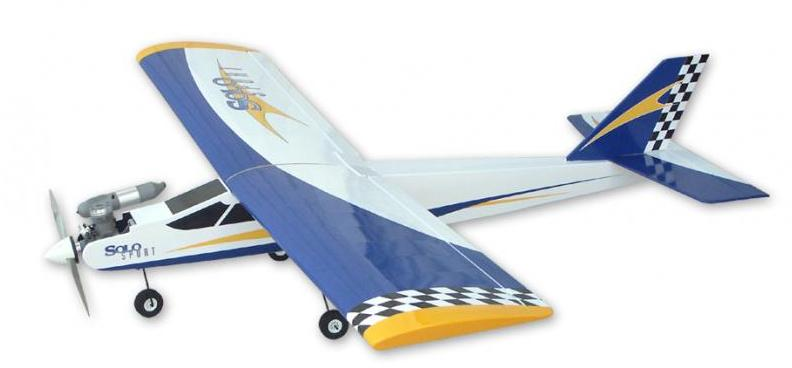
\includegraphics[height=2.5cm]{png/avion} &&
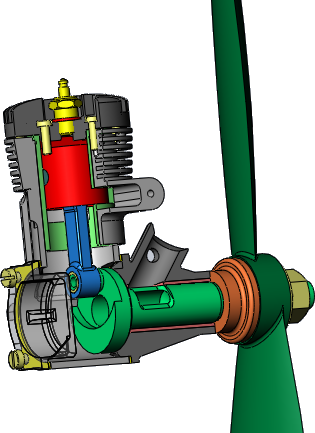
\includegraphics[height=3.5cm]{png/moteur_3d} && 
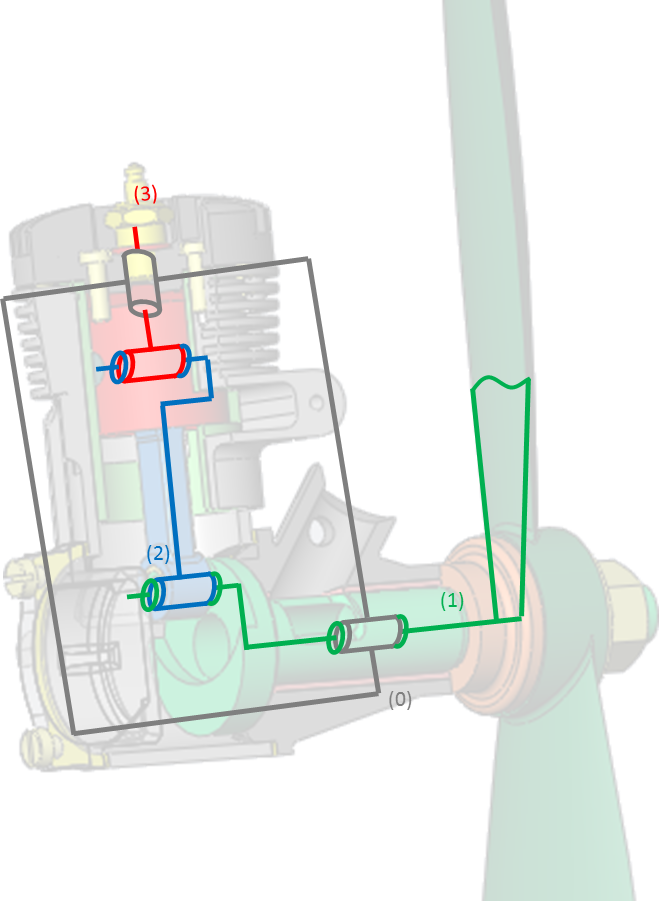
\includegraphics[height=3.5cm]{png/moteur_3d_sch}\\
\textit{Trainer Solo Sport \cite{cite1}} &&
\textit{Modèle CAO d'un} &&
\textit{Modélisation par}\\
 &&
\textit{moteur de modélisme \cite{cite2}} &&
\textit{schéma cinématique}\\
\end{tabular}
\end{center}

\vspace{.2cm}
L'étude des vitesses et des accélérations des points d'un solide est utile pour plusieurs raisons. En phase d'avant projet, par exemple, lors de la phase de conception d'un système mécanique de transmission ou de conversion de mouvement, il est indispensable de connaître la vitesse des solides afin de satisfaire à un cahier des charges.

En phase de dimensionnement des produits, certains composants peuvent être dimensionnés en fonction de la vitesse de fonctionnement du système. Dans d'autres cas, la cinématique est un préalable aux études de dynamique. 

\begin{prob}
\textsc{Problématique :}
\begin{itemize}
\item Comment calculer la vitesse et l'accélération d'un point d'un solide ?
\item Comment établir la loi entrée -- sortie d'un mécanisme ?
\end{itemize}
\end{prob}

\begin{savoir}
\textsc{Savoirs :}
\begin{itemize}
\item Déterminer la trajectoire d'un point par rapport à un autre solide
\item Déterminer les vecteurs vitesse et accélération d'un solide par rapport à un autre solide.
\item Dériver des vecteurs
\end{itemize}
\end{savoir}

\setlength{\parskip}{0ex plus 0.2ex minus 0ex}
 \renewcommand{\contentsname}{}
 \renewcommand{\baselinestretch}{1}

% \vspace{1cm}
\textit{Ce document est en évolution permanente. Merci de signaler toutes
erreurs ou coquilles.}

\tableofcontents

 \renewcommand{\baselinestretch}{1.2}
\setlength{\parskip}{2ex plus 0.5ex minus 0.2ex}





\section{Trajectoire d'un point dans un mécanisme}

\begin{defi}
\textbf{Trajectoire d'un point dans l'espace}

Soit un point $P$ se déplaçant dans un repère $\mathcal{R}_0$. La trajectoire du point $P$ est définie par la courbe $\mathcal{C}(t)$ paramétrée par le temps $t$. On a : 
$$
\forall t\in \mathbb{R}^+, \vect{OM(t)}=
\left[
\begin{array}{l}
x(t)\\
y(t)\\
z(t)\\
\end{array}
\right]_{\mathcal{R}_0}
=x(t)\vect{x_0}+y(t)\vect{y_0}+z(t)\vect{z_0}
$$
\end{defi}


\begin{exemple}
\textit{Moteur de modélisme}

\begin{center}
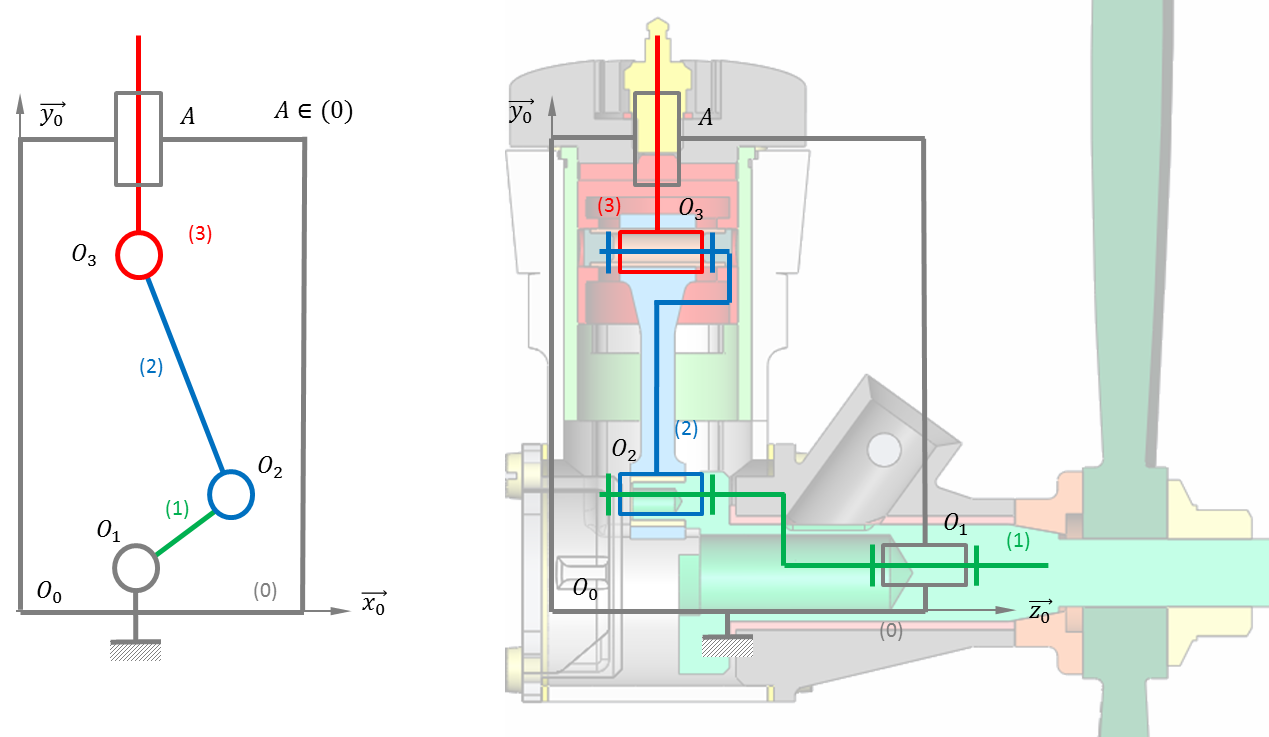
\includegraphics[width=.75\textwidth]{png/moteur_2d_sch}
\end{center}
\begin{center}
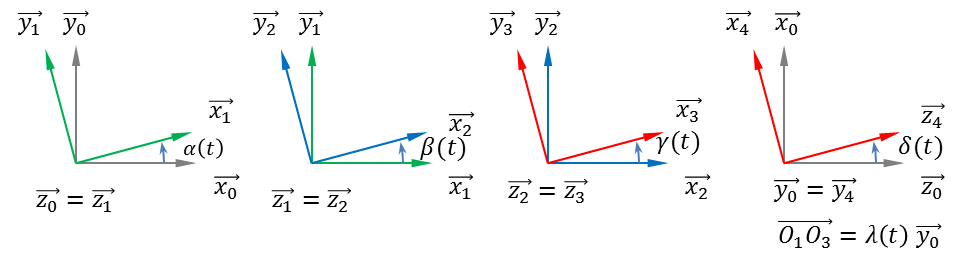
\includegraphics[width=.85\textwidth]{png/param}
\end{center}

Position du point $O_1$ par rapport au point $O_0$ dans le repère $\mathcal{R}_0$ : 
$$
\vect{O_0 O_1}(t)= a\vect{x_0}+b\vect{y_0}+c\vect{z_0}
$$

Position du point $O_2$ par rapport au point $O_1$ dans le repère $\mathcal{R}_1$ : 
$$
\vect{O_1 O_2}(t)= d\vect{x_1}
$$

Le point $O_2$ est donc immobile dans le repère $\mathcal{R}_1$.

Position du point $O_2$ par rapport au point $O_1$ dans le repère $\mathcal{R}_0$ : 
$$
\vect{O_1 O_2}(t)= d\vect{x_1}=d\cos\alpha(t)\vect{x_0}+d\sin\alpha(t)\vect{y_0}
$$

Le point $O_2$ décrit donc un cercle dans le repère $\mathcal{R}_0$.

\end{exemple}



\section{Vecteurs vitesses}
\subsection{Vitesse d'un point appartenant à un solide}

\begin{defi}
\textbf{Vitesse d'un point appartenant à un solide}

Soit un solide $S_0$ auquel on associe le repère $\mathcal{R}_0$ $\left(O_0;\vect{x_0};\vect{y_0};\vect{z_0} \right)$.  Soit un solide $S_1$ auquel on associe le repère $\mathcal{R}_1$,  $\left(O_1;\vect{x_1};\vect{y_1};\vect{z_1} \right)$. Le solide $S_1$ est en mouvement par rapport au solide $S_0$. 

Soit un point $P$ appartenant au solide $S_1$. La vitesse du point $P$ appartenant au solide $S_1$ par rapport au solide $S_0$ se calcule donc ainsi : 
$$
\vect{V(P\in S_1/S_0)}(t) = \left[\dfrac{d\vect{OP(t)}}{dt}\right]_{\mathcal{R}_0}
$$
\end{defi}

\begin{warn}
\begin{minipage}[c]{.15\linewidth}
\begin{center}

\includegraphics[width=.8\textwidth]{png/warning3}
\end{center}
\end{minipage} \hfill
\begin{minipage}[c]{.8\linewidth}
\begin{itemize}
\item Attention à respecter rigoureusement la notation.
\item La vitesse dépend du point d'application.
\end{itemize}
\end{minipage}
\end{warn}

\begin{rem}
\begin{minipage}[c]{.65\linewidth}
Lorsqu'un point est confondu pour deux solides (centre d'une liaison pivot ou d'une liaison rotule par exemple) les vitesses sont égales ainsi, ici : 
$$
\vect{V(0_2\in S_1/S_0)}(t) = \vect{V(0_2\in S_2/S_0)}(t)
$$
\end{minipage}\hfill
\begin{minipage}[c]{.3\linewidth}
\begin{center}
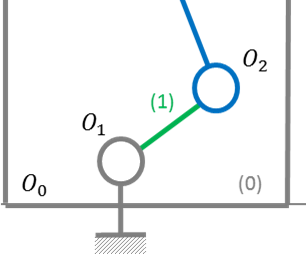
\includegraphics[width=.8\textwidth]{png/2solides}
\end{center}
\end{minipage}
\end{rem}

\begin{exemple}
\textit{Expression de la vitesse du point $O_2$ appartenant à $S_2$ dans le repère $\mathcal{R}_0$.}

$$
\vect{V(O_2\in S_2/S_0)}(t) 
= \left[\dfrac{d\vect{O_0 O_2}}{dt}\right]_{\mathcal{R}_0}
= \underbrace{\left[\dfrac{d\vect{O_0 O_1}}{dt}\right]_{\mathcal{R}_0}}_{\vect{0}}+ \left[\dfrac{d\vect{O_1 O_2}}{dt}\right]_{\mathcal{R}_0}
=\left[\dfrac{d\vect{O_1 O_2}}{dt}\right]_{\mathcal{R}_0}
$$

$$
\vect{V(O_2\in S_2/S_0)}(t) 
=\left[\dfrac{d \; d\vect{x_1}}{dt}\right]_{\mathcal{R}_0}
=d\left[\dfrac{ d\vect{x_1}}{dt}\right]_{\mathcal{R}_0}
=d\left[\dfrac{ d\left(
\cos\alpha(t)\vect{x_0}+\sin\alpha(t)\vect{y_0}
\right)
}{dt}\right]_{\mathcal{R}_0}
$$

$$
\vect{V(O_2\in S_2/S_0)}(t) 
=d\left[
\dfrac{d\cos\alpha(t)}{dt} \cdot \vect{x_0}
+\cos\alpha(t)\cdot \underbrace{\dfrac{d\vect{x_0}}{dt}}_{\vect{0}}
+\dfrac{d\sin\alpha(t)}{dt} \cdot \vect{y_0}
+\sin\alpha(t)\cdot \underbrace{\dfrac{d\vect{y_0}}{dt}}_{\vect{0}}
\right]
$$

$$
\vect{V(O_2\in S_2/S_0)}(t) 
=d\left[
-\dot{\alpha}(t)\sin\alpha(t) \cdot \vect{x_0}
+\dot{\alpha}(t)\cos\alpha(t) \cdot \vect{y_0}
\right]
=d\dot{\alpha}(t)\vect{y_1}
$$


\end{exemple}

\subsection{Vitesse instantanée de rotation}
\begin{defi}
\textbf{Vitesse instantanée de rotation}

Soit un solide $S_0$ auquel on associe le repère $\mathcal{R}_0$ $\left(O_0;\vect{x_0};\vect{y_0};\vect{z_0} \right)$.  Soit un solide $S_1$ auquel on associe le repère $\mathcal{R}_1$,  $\left(O_1;\vect{x_1};\vect{y_1};\vect{z_1} \right)$. Le solide $S_1$ est en mouvement par rapport au solide $S_0$. 

Les 3 rotations sont paramétrées par les angles d'Euler $(\psi;\vect{z_0})$, $(\theta;\vect{u})$, $(\varphi;\vect{z_1})$.

On appelle $\vect{\Omega(S_1/S_0)}$ le vecteur définit ainsi :
$$
\vect{\Omega(S_1/S_0)} = \dot{\psi}\cdot\vect{z_0}+\dot{\theta}\cdot\vect{u}+\dot{\varphi}\cdot\vect{z_1}
$$
\end{defi}

\begin{rem}
\begin{itemize}
\item Attention aux dérivées : $\dot{\psi}$, $\dot{\theta}$ et $\dot{\varphi}$ sont les dérivées des positions angulaires. Elles sont donc exprimées en $rad/s$.
\item Le vecteur instantané de rotation est indépendant du point d'application.
\item On a la relation suivante :
$$\vecto{S_1}{S_0} = -\vecto{S_0}{S_1}$$
\end{itemize}
\end{rem}

\begin{exemple}

\textit{Calcul de $\vect{\Omega(S_1/S_0)}$ et $\vect{\Omega(S_2/S_1)}$}

\begin{minipage}[c]{.3\linewidth}
\begin{center}
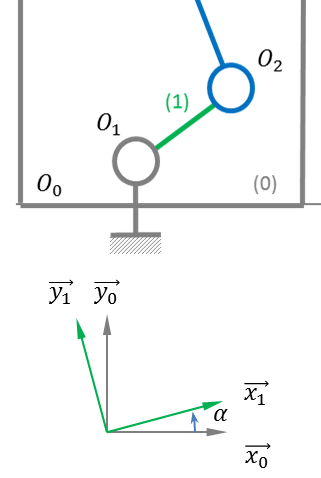
\includegraphics[width=.8\textwidth]{png/omega}
\end{center}
\end{minipage}
\hfill
\begin{minipage}[c]{.6\linewidth}
Lorsque deux solides sont en liaison et que cette dernière est paramétrée, la détermination de $\vect{\Omega(S_1/S_0)}$ est immédiate : 
$$
\vect{\Omega(S_1/S_0)}=\dot{\alpha}\vect{z_0}
$$
De même, 
$$
\vect{\Omega(S_2/S_1)}=\dot{\beta}\vect{z_0}
$$
\end{minipage}
\end{exemple}

\subsection{Dérivation vectorielle}
\begin{exemple}
\textit{Calcul de $\vect{V(O_2\in S_2/S_0)}(t)$.}

On a vu que pour calculer ce vecteur, il était nécessaire de :
\begin{enumerate}
\item utiliser le théorème de Chasles pour exprimer le vecteur $\vect{O_1 O_2}$;
\item projeter le vecteur $\vect{x_1}$ dans le repère $\mathcal{R}_0$ pour pouvoir le dériver; 
\item dériver ensuite l'expression obtenue.
\end{enumerate}

Cette procédure s'avère donc très calculatoire et va devenir très lourde en calcul dès lors que le nombre de solides et de projections vont se multiplier.

\textit{Calculons par exemple $\vect{V(O_3\in S_3/S_0)}(t)$.}

D'une part, 
$$\vect{V(O_3\in S_3/S_0)}(t) 
= \left[\dfrac{d\vect{O_1O_3}}{dt}\right]_{\mathcal{R}_0}
= \underbrace{\left[\dfrac{d\vect{O_1A}}{dt}\right]_{\mathcal{R}_0}}_{=\vect{0}}
+ \left[\dfrac{d\vect{AO_3}}{dt}\right]_{\mathcal{R}_0}=
-\dot{\lambda} \vect{y_0}
$$

D'autre part, 
$$
\vect{V(O_3\in S_3/S_0)}(t) 
= \left[\dfrac{d\vect{O_1O_3}}{dt}\right]_{\mathcal{R}_0}
= \underbrace{\left[\dfrac{d\vect{O_1O_2}}{dt}\right]_{\mathcal{R}_0}}_{\vect{V(O_2\in S_2/S_0)}(t) }
+ \left[\dfrac{d\vect{O_2O_3}}{dt}\right]_{\mathcal{R}_0}
$$
Calculons donc $\left[\dfrac{d\vect{O_2O_3}}{dt}\right]_{\mathcal{R}_0}$.
$$
\left[\dfrac{d\vect{O_2O_3}}{dt}\right]_{\mathcal{R}_0}
= \left[\dfrac{d \left( f \vect{x_2} \right)}{dt}\right]_{\mathcal{R}_0}
= f\left[\dfrac{d \vect{x_2}}{dt}\right]_{\mathcal{R}_0}
$$

Pour dériver $\vect{x_2}$, il est alors nécessaire de le projeter dans $\mathcal{R}_0$ : 
$$
\vect{x_2}
=\cos\beta\vect{x_1}+\sin\beta\vect{y_1}
=\cos\beta\left( \cos\alpha\vect{x_0}+\sin\alpha\vect{y_0}\right)
+\sin\beta\left( \cos\alpha\vect{y_0}-\sin\alpha\vect{x_0}\right)
$$
$$
\vect{x_2}
=
\cos\beta\cos\alpha\vect{x_0}
+\cos\beta\sin\alpha\vect{y_0}
+\sin\beta\cos\alpha\vect{y_0}
-\sin\beta\sin\alpha\vect{x_0}
$$
On a donc :
\begin{eqnarray*}
\left[\dfrac{d \vect{x_2} }{dt}\right]_{\mathcal{R}_0}
&=&-\dot{\beta}\sin\beta\cos\alpha\vect{x_0}
-\dot{\alpha}\cos\beta\sin\alpha\vect{x_0}\\
&&-\dot{\beta}\sin\beta\sin\alpha\vect{y_0}
+\dot{\alpha}\cos\beta\cos\alpha\vect{y_0}\\
&&+\dot{\beta}\cos\beta\cos\alpha\vect{y_0}
-\dot{\alpha}\sin\beta\sin\alpha\vect{y_0}\\
&&-\dot{\beta}\cos\beta\sin\alpha\vect{x_0}
-\dot{\alpha}\sin\beta\sin\alpha\vect{x_0}
\end{eqnarray*}

Reste ensuite à substituer les termes pour calculer $\vect{V(O_3\in S_3/S_0)}(t)$.

Cette expression bien que lourde serait néanmoins simplifiable en l'exprimant dans la base adéquate.

\textit{NB :} dans ce cas, la chaîne de solides est fermée, il faudrait identifier les deux expressions de $\vect{V(O_3\in S_3/S_0)}(t)$. Les projections suivant $\vect{x_0}$ sont donc nulles.
\end{exemple}

En cinématique, le recours à la dérivation dans des bases différentes est systématique.
Dans la mesure du possible, on évitera toujours de projeter les vecteurs dans la base fixe. On conservera ainsi des expressions vectorielles simplifiées.
La méthode pour calculer des dérivées sera donc la suivante.

\begin{resultat}
\textbf{Dérivation vectorielle}

Soient $\mathcal{R}_0$ et $\mathcal{R}_1$ deux repères orthonormés directs. Soit $\vect{v}$ un vecteur de l'espace. On note $\vect{\Omega(\mathcal{R}_1/\mathcal{R}_0)}$ le vecteur instantané de rotation permettant d'exprimer les rotations entre chacune des deux bases. 

La dérivée d'un vecteur dans une base mobile se calcule donc ainsi :

$$
\left[\dfrac{d\vect{v}}{dt}\right]_{\mathcal{R}_0} =
\left[\dfrac{d\vect{v}}{dt}\right]_{\mathcal{R}_1} 
+ \vect{\Omega(\mathcal{R}_1/\mathcal{R}_0)}\wedge \vect{v}
$$
\end{resultat}

\begin{methode}
\textbf{Calcul du produit vectoriel -- Méthode analytique}

Soient $\vect{v_1}$ et $\vect{v_2}$ deux vecteurs exprimés dans $\mathcal{R}_0$. 

On a alors :
$$
||\vect{v_1} \wedge \vect{v_2}|| = ||\vect{v_1}|| \cdot ||\vect{v_2}|| \cdot \sin \left(\vect{v_1};\vect{v_2} \right) 
$$

Le vecteur résultant du produit vectoriel de ces deux vecteurs est orthogonal au plan formé par $\vect{v_1}$ et $\vect{v_2}$. $\vect{v_1}$, $\vect{v_2}$ et le vecteur résultant doivent former un trièdre direct. 

On a :
$$
\vect{v_1} \wedge \vect{v_2} 
= 
\left[
\begin{array}{c}
v_{1x}\\
v_{1y}\\
v_{1z}\\
\end{array}
\right]_{\mathcal{R}_0}
\wedge
\left[
\begin{array}{c}
v_{2x}\\
v_{2y}\\
v_{2z}\\
\end{array}
\right]_{\mathcal{R}_0}
=
\left[
\begin{array}{c}
v_{1y}v_{2z}-v_{1z}v_{2y}\\
-\left( v_{1x}v_{2z}-v_{1z}v_{2x}\right)\\
v_{1y}v_{2y}-v_{1y}v_{2x}\\
\end{array}
\right]_{\mathcal{R}_0}
$$


\begin{minipage}[c]{.15\linewidth}
\begin{center}

\includegraphics[width=.8\textwidth]{png/warning3}
\end{center}
\end{minipage} \hfill
\begin{minipage}[c]{.8\linewidth}
Pour réaliser le produit vectoriel, les vecteurs doivent être exprimés dans le même repère.
\end{minipage}
\end{methode}

\begin{methode}
\textbf{Calcul du produit vectoriel -- Méthode graphique}

Cette méthode sera utilisée lors du produit vectoriel entre vecteurs normés. Le calcul du produit vectoriel est alors déduit de la lecture des figures planes : 

\begin{minipage}[c]{.3\linewidth}
\begin{center}
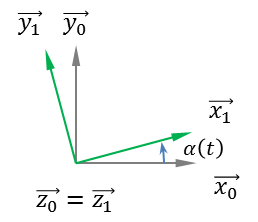
\includegraphics[width=.9\textwidth]{png/alpha}
\end{center}
\end{minipage} \hfill
\begin{minipage}[c]{.65\linewidth}
$$
\vect{x_0}\wedge\vect{y_0}=\vect{z_0}
$$
$$
\vect{x_0}\wedge\vect{x_1}=
\underbrace{+}_{\vect{x_0} { et }\vect{x_1}} 
\underbrace{\sin \alpha(t)}_{\text{angle entre} \vect{x_0} \text{ et }\vect{x_1}} 
\underbrace{\vect{z_0}}_{\text{Vecteur normal à } \vect{x_0} \text{ et }\vect{x_1}}
$$
$$
\vect{y_0}\wedge\vect{x_1}
=- \sin\left( \pi/2 - \alpha(t)\right) \vect{z_0}
=- \cos \alpha(t) \vect{z_0}
$$
\end{minipage}

\end{methode}

\begin{exemple}
\textit{Calcul de $\left[\dfrac{d\vect{x_2}}{dt}\right]_{\mathcal{R}_0}$ et $\left[\dfrac{d\vect{x_3}}{dt}\right]_{\mathcal{R}_0}$. On donne :}
$$\vect{\Omega(S_2/S_0)} = 
\left( \dot{\alpha} + \dot{\beta} \right)\vect{z_0}
\quad
\vect{\Omega(S_3/S_0)} = 
\left( \dot{\alpha} + \dot{\beta} + \dot{\gamma} \right)\vect{z_0}
$$

\begin{minipage}[c]{.65\linewidth}
$$
\left[\dfrac{d\vect{x_2}}{dt}\right]_{\mathcal{R}_0} 
= \underbrace{\left[\dfrac{d\vect{x_2}}{dt}\right]_{\mathcal{R}_2}}_{\vect{0}}
+ \vect{\Omega(S_2/S_0)} \wedge \vect{x_2}
=  \left( \left( \dot{\alpha} + \dot{\beta} \right)\vect{z_0} \right)\wedge \vect{x_2}
$$
On utilise alors la seconde figure plane où figurent $\vect{z_0}=\vect{z_1}$ et $\vect{x_2}$. 
$$
\left[\dfrac{d\vect{x_2}}{dt}\right]_{\mathcal{R}_0} 
=  \left(  \dot{\alpha} + \dot{\beta} \right)\vect{z_0}\wedge \vect{x_2}
=  \left(  \dot{\alpha} + \dot{\beta} \right)\vect{y_2}
$$
\end{minipage}\hfill
\begin{minipage}[c]{.3\linewidth}
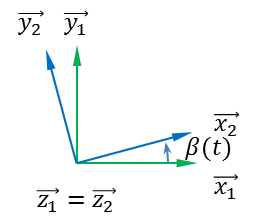
\includegraphics[width=.9\textwidth]{png/beta}
\end{minipage}

\vspace{0.5cm}

\begin{minipage}[c]{.65\linewidth}
$$
\left[\dfrac{d\vect{x_3}}{dt}\right]_{\mathcal{R}_0} = 
\underbrace{\left[\dfrac{d\vect{x_3}}{dt}\right]_{\mathcal{R}_3}}_{\vect{0}}
+ \vect{\Omega(S_3/S_0)} \wedge \vect{x_3}
$$
$$
\left[\dfrac{d\vect{x_3}}{dt}\right]_{\mathcal{R}_0} 
= \left(\left( \dot{\alpha} + \dot{\beta} + \dot{\gamma} \right)\vect{z_0} \right) \wedge \vect{x_3}
= \left( \dot{\alpha} + \dot{\beta} + \dot{\gamma} \right)\vect{y_3}
$$
\end{minipage}\hfill
\begin{minipage}[c]{.35\linewidth}
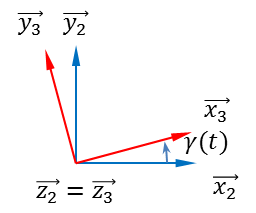
\includegraphics[width=.9\textwidth]{png/gamma}
\end{minipage}
\vspace{0.5cm}
\end{exemple}

\subsection{Calcul de la loi Entrée -- Sortie dans une chaîne de solides fermée}
\begin{methode}
Un système se présentant sous forme d'une chaîne de solide fermée a pour but de transformer un mouvement. On s'intéresse alors pour cela à la relation cinématique liant le mouvement d'entrée du système et le mouvement de sortie. On écrit pour cela une \textbf{fermeture de chaîne géométrique}. Pour cela :
\begin{enumerate}
\item paramétrer le mécanisme;
\item identifier la grandeur d'entrée et de sortie;
\item à l'aide du théorème de Chasles, exprimer le vecteur nul en fonction des vecteurs liant le centre de chacune des liaisons;
\item projeter la relation vectorielle sur une des bases;
\item combiner les relations pour exprimer la sortie en fonction de l'entrée;
\item dériver si besoin pour avoir le lien entre les vitesses. 
\end{enumerate}
\end{methode}


\begin{exemple}

\begin{minipage}[c]{.6\linewidth}
Le système a été paramétré. 

Dans le cas d'un système bielle-manivelle comme le moteur de modélisme, on veut connaître la vitesse de rotation de l'hélice $\dot{\alpha}(t)$ en fonction de la vitesse de translation du piston $\dot{\lambda}(t)$. 

La fermeture géométrique est donc la suivante : 
\begin{eqnarray*}
\vect{O_1 O_2} + \vect{O_2 O_3} +\vect{O_3 O_1} = \vect{0} \\
\Longleftrightarrow d\vect{x_1} + e \vect{x_2} - \lambda \vect{y_0}  = \vect{0}
\end{eqnarray*}

Avant de projeter la relation vectorielle sur le repère $\mathcal{R}_0$, exprimons l'angle $\varphi(t)$ en fonction de $\alpha(t)$ et $\beta(t)$:
$$
\varphi + \left(\pi-\beta\right)+\left(\dfrac{\pi}{2}-\alpha\right) = \pi 
\Longleftrightarrow
\varphi = \beta+\alpha-\dfrac{\pi}{2}
$$
\end{minipage}\hfill
\begin{minipage}[c]{.35\linewidth}
\begin{center}
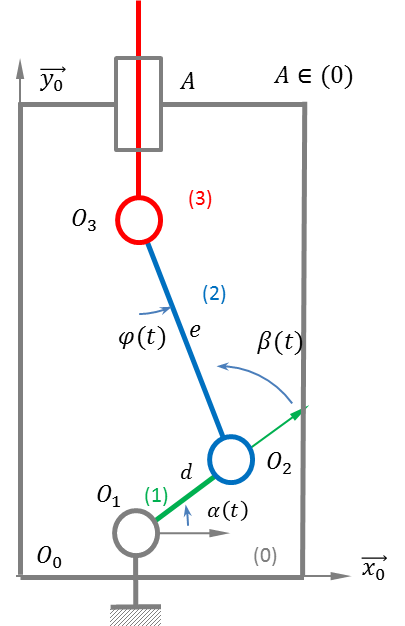
\includegraphics[width=.9\textwidth]{png/chaine}
\end{center}
\end{minipage}

En projetant l'équation vectorielle sur $\vect{x_0}$ et $\vect{y_0}$ on a : 
$$
\left\{
\begin{array}{l}
d\cos\alpha - e \sin \varphi = 0 \\
d\sin\alpha + e \cos \varphi - \lambda= 0 \\
\end{array}
\right.
\Longleftrightarrow 
\left\{
\begin{array}{l}
\sin \varphi = \dfrac{d\cos\alpha}{e}  \\
\cos \varphi = \dfrac{\lambda - d\sin\alpha}{e} \\
\end{array}
\right.
$$

En passant au carré et en sommant les deux expressions, on a donc : 
$$
\left(\dfrac{d\cos\alpha}{e}\right)^2 + \left(\dfrac{\lambda - d\sin\alpha}{e}\right)^2 = 1 
\Longleftrightarrow
d^2\cos^2\alpha + \lambda^2 + d^2\sin^2\alpha +2d\lambda\sin\alpha = e^2
$$

$$
\Longleftrightarrow
d^2+ \lambda^2 +2d\lambda\sin\alpha = e^2
$$
Pour exprimer $\lambda$ en fonction de $\alpha$, il faut donc résoudre une équation du second degré. Pour exprimer $\alpha$ en fonction de $\lambda$, la méthode est directe. 

%Résolvons donc 
%$$
%\lambda^2 +2d\lambda\sin\alpha +d^2- e^2=0
%$$
%On calcule le discriminant :
%$$
%\Delta = 4d^2\sin^2\alpha-4\left( d^2- e^2\right)
%$$

%On a donc 
%$$
%\lambda 
%= \dfrac{-2d\sin\alpha \pm \sqrt{\Delta}}{2}
%= -d\sin\alpha \pm \sqrt{d^2\sin^2\alpha-\left( d^2- e^2\right)}
%$$
\end{exemple}

\begin{methode}
\textbf{Méthodes pour manipuler les systèmes équations :} 
\begin{enumerate}
\item Pour supprimer $\lambda$ : on met les deux équations sous la forme $\lambda =$ et on fait le rapport des deux équations.
\item Pour supprimer $\varphi$ : on met une équation sous la forme $\cos\varphi = $ et la seconde sous la forme $\cos\varphi = $ et on utilise la relation $\cos^2\varphi +\sin^2\varphi =1 $.
\item Dans d'autres cas, on peut avoir à utiliser l'expression de la tangente.
\end{enumerate}
\end{methode}
\section{Accélération d'un point appartenant à un solide}
\begin{defi}
\textbf{Accélération d'un point appartenant à un solide}

Soit un solide $S_0$ auquel on associe le repère $\mathcal{R}_0$ $\left(O_0;\vect{x_0};\vect{y_0};\vect{z_0} \right)$.  Soit un solide $S_1$ auquel on associe le repère $\mathcal{R}_1$,  $\left(O_1;\vect{x_1};\vect{y_1};\vect{z_1} \right)$. Le solide $S_1$ est en mouvement par rapport au solide $S_0$. 


Soit un point $P$ appartenant au solide $S_1$. L'accélération du point $P$ appartenant au solide $S_1$ par rapport au solide $S_0$ se calcule donc ainsi : 
$$
\vect{\Gamma(P\in S_1/S_0)}(t) = \left[\dfrac{d\left( \vect{V(P\in S_1/S_0)}(t)\right)}{dt}\right]_{\mathcal{R}_0}
$$

\end{defi}
\begin{exemple}
\textbf{Calcul de $\vect{\Gamma(O_2\in S_1/S_0)}(t)$}
$$\vect{\Gamma(O_2\in S_1/S_0)}(t)
=\left[\dfrac{\vect{V(O_2\in S_1/S_0)}(t)}{dt}\right]_{\mathcal{R}_0}
=\left[
\dfrac{d\dot{\alpha}\vect{y_1}}{dt}
\right]_{\mathcal{R}_0}
$$

$$\vect{\Gamma(O_2\in S_1/S_0)}(t)
=
d\ddot{\alpha}\vect{y_1}-d\dot{\alpha}^2\vect{x_1}
$$

\end{exemple}

\begin{thebibliography}{2}
  \bibitem[1]{cite1} Trainer Solo Sport, \textit{Avio et Tiger}, \url{http://www.net-loisirs.com/trainer-solo-sport-p1155.html}.

\bibitem[2]{cite2} Université Bretagne Sud, \textit{Moteur de modélisme} \url{http://foad.univ-ubs.fr/file.php/1355/TP_meca3d/Moteur_modelisme.zip}

%\bibitem[3]{cite3} \url{http://www.aquadesign.be/actu/article-2535.php}
\end{thebibliography}
\end{document}
